\section{The N2Sky Architecture}\label{TheN2SkyArchitecture}

\subsection{Current Architecture Analysis}\label{CurrentArchitectureAnalysis}
\subsubsection{Architecture design}\label{Architecturedesign}
\subsubsection{Components}\label{Components}
\subsubsection{Current User Interface}\label{CurrentUserInterface}
\subsubsection{Usability and user experience}\label{Usabilityanduserexperience}



\subsection{Redesign motivation}\label{Redesignmotivation}

Application redesign is a project, which takes a lot of work. But at some point every designer faced a refactoring project. It has a lot to do with user experience. Bad user experience will make users stop use an application and leave negative feedback on application in general. 

\subsubsection{Redesign Process }\label{Redesign Process}

There is data, information and user experience of previous version of N2Sky to work with. Making redesign it is already known who the users are and what they trying to achieve.  Using this information it is possible to build an aims for a future user interface and user experience.


\begin{description}

\item[Finding problems]  N2Sky user interface is not intuitive understandable. 
\begin{figure}[htbp]
\begin{center}
  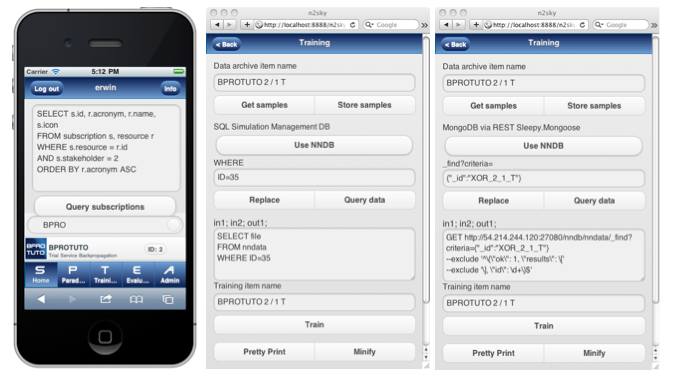
\includegraphics[width=\linewidth]{components/2/old_arch.png}
  \caption{Current N2Sky User Interface}
  \label{fig:old_arch}
\end{center}
\end{figure}

\end{description}


\subsubsection{Refactoring the User Interface}\label{Refactoring the User Interface}
\subsubsection{Introducing a new User Experience Design}\label{Introducing a new User Experience Design}
\subsubsection{Services adoption}\label{Services adoption}


\subsection{Contemporary N2Sky Architecture}\label{ContemporaryN2SkyArchitecture}
\subsubsection{Conceptual user interface}\label{Conceptual user interface}	

\subsection{Technology Stack}\label{Technology Stack}
